\documentclass{article}

\usepackage[dblblindworkshop]{neurips_2026}
\workshoptitle{Interpretability as a Science, NeurIPS 2026}

\usepackage[utf8]{inputenc}
\usepackage[T1]{fontenc}
\usepackage{amsmath}
\usepackage{amssymb}
\usepackage{booktabs}
\usepackage{float}
\usepackage{graphicx}
\usepackage{microtype}
\usepackage{xcolor}
\usepackage{url}
\usepackage{hyperref}
\hypersetup{hidelinks}

\title{Beyond Short Names: Emoji Keyword Retrieval across Models\\
and a Bounded Late-Component Test}

\author{Anonymous Authors}

\newcommand{\topone}{\operatorname{top1}}
\newcommand{\codepoint}{\textsc{codepoint}}
\newcommand{\alias}{\textsc{keyword}}

\begin{document}

\maketitle

\begin{abstract}
We use a prospectively specified two-arm design to distinguish cross-model
lexical readability from a component-level causal account. Text language
models receive emoji as Unicode token sequences rather than rendered
pictures. The observational arm crosses 55 emoji and 55 non-emoji Unicode
symbols with raw, official-name, word-disjoint CLDR-keyword, and literal
codepoint views. Across nine prespecified model--tokenizer configurations, the
emoji keyword-minus-codepoint retrieval effect is positive in unrestricted
and exact four-view token-count-matched analyses. Every configuration exceeds
the registered 0.02 floor, and the four-model partial-conjunction primary
passes ($p=0.0027$). The symbol comparison recovers official names broadly and
finds smaller, heterogeneous keyword effects. The passed observational
criterion admits a causal arm in Llama 3.2 3B: rank-8 subspaces learned from
128 source emoji are tested at six late attention and MLP outputs on 192
held-out emoji. Engineering controls reproduce the baseline exactly. No
primary site satisfies the joint necessity-and-sufficiency criterion under
this single-context, low-baseline test. The lexical relation holds in all nine
prespecified configurations. The bounded late-component account remains
unsupported.
\end{abstract}

\section{Introduction}

Readers encounter emoji as compact visual objects. A text language model
instead receives encoded Unicode scalars and tokenizer-dependent sequences.
An official label may therefore be recoverable because it co-occurs with the
character in standards, documentation, or training data. That observation
alone cannot establish rendered-glyph perception, a human-like concept, or a
localized semantic circuit.

Single-codepoint emoji nevertheless make the recoverability question
unusually clean. Under the word-disjointness constraint below, the character
shares no substring, no morpheme, and not one ASCII-alphanumeric word with the
keyword it must retrieve, so any observed relation must be carried by learned
association rather than by surface form. Atomic Unicode characters thereby
offer a controlled testbed for how text-only models attach lexical relations
to opaque tokens, and a concrete auditing target for multilingual and
social-media systems that consume such tokens at scale.

A prospectively specified two-arm design separates two narrower questions.
The observational arm asks whether a raw atomic emoji retrieves a
word-disjoint CLDR keyword better than its literal \texttt{U+...} spelling
after exact token-count matching. Conditional on that result, the causal arm
asks whether a low-rank late-component intervention identifies a
representation that is both necessary and sufficient for the relation. This
design yields an auditable distinction between broad lexical readability and
one simple mechanistic account; it makes no claim of visual perception or
human-like emoji understanding.

The study is organized around three safeguards and their corresponding
results:

\begin{itemize}
  \item Four text views and three disjoint item sets separate the raw Unicode
  surface, official English CLDR name, word-disjoint CLDR keyword, and literal
  codepoint spelling. The causal source and evaluation sets receive no
  observational-arm evaluation, although their surfaces may have appeared in
  earlier studies.
  \item The observational primary passes: 4/4 core configurations and 9/9
  total configurations are positive in unrestricted and exact four-view
  token-count-matched analyses. The cross-model partial-conjunction value is
  $0.0027$.
  \item A conditionally admitted causal experiment passes all zero-hook and
  restoration controls and finds no primary block-24 attention or MLP output
  that is jointly necessary and sufficient. A secondary block-27 MLP patch
  raises the composite endpoint through keyword gains and codepoint losses;
  its necessity criterion fails.
\end{itemize}

The observational result extends beyond exact-short-name retrieval under the
prespecified endpoint. The causal result rejects one prespecified rank-8
late-component mechanism. Distributed, redundant, nonlinear, and
item-private explanations remain unresolved.

\section{Related work}

\paragraph{Textual sources of emoji meaning.}
Emoji representations have been learned from descriptions
\citep{eisner2016emoji2vec}, linked to lexical sense inventories
\citep{wijeratne2017emojinet}, and induced from usage through emoji prediction
\citep{felbo2017deepmoji,barbieri2018interpretable}. These approaches identify
descriptions, lexical resources, and context as distinct sources of emoji
meaning. We use CLDR names and keywords \citep{unicode2026cldr} as
source-auditable endpoints and ask which item-wise textual relations are
recoverable from a raw Unicode input. Co-occurrence with these resources
remains a candidate explanation for every positive result.

\paragraph{Probing and tokenizer controls.}
Probe accuracy can reflect the diagnostic model or its control task
\citep{hewitt2019designing}, and tokenizer choice can materially change model
comparisons \citep{rust2021tokenizer}. Our item-wise nearest-neighbor readout
avoids a learned diagnostic classifier. Unrestricted and exact four-view
token-count-matched tests address length while leaving token identity and
tokenizer construction uncontrolled. The readout also differs from
whole-representation similarity measures such as CKA
\citep{kornblith2019similarity}: it asks whether the correct item is the
nearest partner across two text views.

\paragraph{Causal intervention.}
Conventional probing performance need not measure how information is used
\citep{elazar2021amnesic}. Causal mediation, interchange interventions, and
model editing instead test whether internal variables affect computation
\citep{vig2020causal,geiger2021causal,meng2022rome}. Optimization-based
alignment methods go further and learn the intervention subspace itself,
either by maximizing interchange accuracy
\citep{geiger2024das,wu2023boundless} or through sparse dictionary features
\citep{bricken2023monosemanticity,cunningham2024sparse}. Our component test
follows the causal distinction while fixing the subspace by a closed-form
cross-covariance rule before any evaluation forward: a prespecified site must
pass random-adjusted necessity and sufficiency on a disjoint evaluation set.
It therefore rejects one fixed account rather than the best discoverable one,
a bound Section~6 records. We retain the resulting negative test without
adapting the layer, rank, or endpoint.

\section{Prospective design}
\label{sec:design}

\subsection{Input views and disjoint item sets}

For auditability, we retain two internal study labels. \textbf{T19-L}
denotes the observational lexical-retrieval arm (``L'' for lexical), and
\textbf{T19-C} denotes the conditionally admitted component-causal arm.
They are labels for the two arms defined below; no knowledge of the preceding
project sequence is required. Appendix \ref{app:lineage} gives the short
decision lineage that led to T19-L without treating earlier exploration as
part of its confirmatory evidence.

Throughout, \emph{glyph} means the raw Unicode scalar string supplied to a
text model. No raster image is rendered. Atomic emoji are single-codepoint,
fully-qualified Emoji 17 entries introduced no later than Emoji 13.1
\citep{unicode2025emoji}. For each item, the official-name view is the exact
English CLDR 48.2 \texttt{tts} value; the keyword view is one exact English
CLDR \texttt{default} keyword. After lowercasing and extracting ASCII
\texttt{[a-z0-9]+} words, official-name and keyword word sets must be nonempty
and disjoint. The fourth view is the uppercase literal codepoint spelling.
When several keywords qualify, one deterministic maximum bipartite matching
assigns globally unique labels; a fixed SHA-256 edge order breaks ties before
any T19 model forward.

\begin{table}[t]
\centering
\scriptsize
\setlength{\tabcolsep}{2.5pt}
\begin{tabular}{p{0.17\linewidth}p{0.35\linewidth}p{0.15\linewidth}p{0.20\linewidth}}
\toprule
Raw scalar$^\dagger$ & CLDR \texttt{tts} & Keyword & Literal view \\
\midrule
U+1F923 & rolling on the floor laughing & lmao & \texttt{U+1F923} \\
U+1F928 & face with raised eyebrow & skeptic & \texttt{U+1F928} \\
U+00B4  & acute accent & tone & \texttt{U+00B4} \\
\bottomrule
\end{tabular}
\caption{Concrete prespecified views for two emoji and one non-emoji symbol.
$^\dagger$The model receives the scalar itself; the table names it by codepoint
because the paper typeface need not render every glyph. The literal view is
the displayed ASCII string.}
\label{tab:examples}
\end{table}

The observational set contains 55 emoji and 55 non-emoji Unicode symbols.
Symbols are single scalars in a Unicode general category beginning with
\texttt{S}, have \texttt{Emoji=false}, have valid disjoint CLDR keywords, and
are absent from every strict-UTF-8, no-NUL repository blob at the prespecified
boundary. This is repository-relative freshness, not pretraining novelty.
Exact emoji surfaces may have appeared in earlier experiments; the endpoint,
keyword assignment, and item-set split are prospective, not the emoji surfaces.

Two further sets contain 128 causal-source and 192 causal-evaluation emoji.
All 430 codepoints and 430 keywords are unique across sets. Figure
\ref{fig:design} summarizes the separation and the one-way admission rule.

\begin{figure}[t]
  \centering
  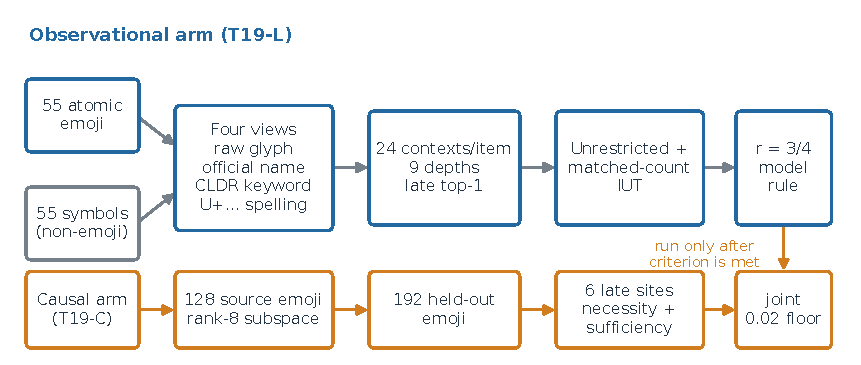
\includegraphics[width=\linewidth]{figures/t19_design.pdf}
  \caption{Prospective T19 design. T19-L crosses two glyph kinds with four
  text views. Only the emoji endpoint enters the registered cross-model
  primary. T19-C runs only after that criterion is met and uses disjoint source and
  evaluation emoji. No causal-set item receives a T19-L forward.}
  \label{fig:design}
\end{figure}

\subsection{Observational readout}

For each item and view, the prespecified evaluation pipeline appends one of two suffix carriers
(\texttt{" a"} or \texttt{" |"}) at distances 1, 2, 4, and 8 and records the
hidden state at the selected suffix token at nine normalized depths. Batch
size is one; no chat template or added special token is used. The primary
late window is fixed at depths $0.75$, $0.875$, and $1.0$, yielding 24
contexts per item.

Within each view and context, hidden states are centered across items and each
row is L2-normalized. Let $z^{v,c}_i$ denote the resulting vector for item $i$,
view $v$, and context $c$. Cross-view top-1 retrieval is

\begin{equation}
  R_c(g \rightarrow v) = \frac{1}{n}\sum_{i=1}^{n}
  \mathbf{1}\left[i = \arg\max_j
  \left\langle z^{g,c}_i, z^{v,c}_j \right\rangle\right].
  \label{eq:retrieval}
\end{equation}

The per-model primary estimate is

\begin{equation}
  \Delta_m = \frac{1}{24}\sum_c
  \left[R_c(g \rightarrow \alias) -
  R_c(g \rightarrow \codepoint)\right]
  \label{eq:primary}
\end{equation}

on the 55 observational emoji. This is a nearest-neighbor readout from hidden
states, not a next-token generation score.

\subsection{Token-count intersection and cross-model test}

Every model must pass two components. The unrestricted component uses all 55
emoji and permutes keyword correspondence within glyph kind. The matched
component retains non-singleton strata sharing the exact four-view
token-count signature and permutes keywords only within stratum. Retrieval in
that component uses the retained pool ($n=31$--$41$ emoji across models), so
its chance level is $1/n$; unrestricted and matched magnitudes are not treated
as directly commensurable. Official-name and codepoint correspondences stay fixed.
Thus the one-sided randomization test asks whether the fixed keyword mapping
beats mappings allowed by its null; because the codepoint term is fixed, it is
not a paired significance test of keyword--codepoint equality. The registered
primary combines that test with the observed comparative requirement
$\Delta_m\geq0.02$ in both components. At $n=55$, the latter requires at least
two net top-1 successes; in the smaller matched pools it requires at least one.
Each component uses 19,999 draws, and the model intersection--union test
(IUT) $p$-value is the maximum of the two component values.

The sole cross-model primary uses four prespecified core configurations: Llama 3.2 3B base,
Qwen2.5 7B base, OLMo 2 1B base, and Gemma 2 2B IT. It tests the partial
conjunction that at least $r=3$ of $m=4$ configurations pass
\citep{benjamini2008partial}. With ordered model IUT values
$p_{(1)}\leq\cdots\leq p_{(4)}$, the registered value is
$p_{\mathrm{PC}}=\min(1,2p_{(3)})$. The other five configurations and all symbol or
official-name results are secondary and cannot admit the causal arm.

We report percentile intervals from 20,000 item bootstrap replicates as
descriptive uncertainty. They are not substituted for the permutation-based
primary decision.

\subsection{Conditionally admitted causal test}

After the observational criterion was committed, T19-C ran in the
prespecified Llama 3.2 3B base configuration. The six sites are the attention
and MLP component outputs at blocks 21, 24, and 27: the tensors returned by
the attention output projection and by the MLP down-projection, hooked before
their residual addition. At each site we learned a rank-8 basis from the left
singular directions of the centered, row-normalized glyph--keyword
cross-covariance on 128 source emoji. The control basis is deterministic
rather than ad hoc: sixteen seeded Gaussian directions inside the source
span are deflated against the learned basis and orthonormalized, and the
first eight are kept. Blocks 24 attention and MLP were primary; blocks 21
and 27 were secondary.

On 192 different evaluation emoji, the two criteria intervene on different
forwards. Necessity intervenes on the glyph forward: with $P$ the learned
rank-8 projector and $\mu$ the source-bank glyph mean at the site, the site
output $g$ is replaced by $g-P(g-\mu)$. Sufficiency intervenes on the
codepoint forward: the site output $c$ is replaced by $c+P(g-c)$, using the
same item's glyph forward, with the replacement cast to BF16 at injection.
Analogous operations in the random basis define adjusted effects:

\begin{align}
N_s &= E_s(\text{random removal})-E_s(\text{learned removal}),\\
S_s &= E_s(\text{learned patch})-E_s(\text{random patch}).
\end{align}

Both source and evaluation inputs append eight copies of the single-token
\texttt{" |"} suffix; the intervention and readout use its first token
(distance 1). The endpoint reads the final hidden state of the intervened
forward at that token as a query against two fixed 192-row galleries built
once from clean, un-intervened forwards: the keyword states and the codepoint
states. Query matrix and each gallery are independently centered by their own
item means, row-normalized, and scored by cosine top-1 identity, giving
$E_s=$ keyword top-1 minus codepoint top-1. The glyph query measures the
baseline and necessity conditions. The patched codepoint query measures
sufficiency; there the codepoint term is self-retrieval and equals 1 at
baseline, so a patch can raise $E_s$ either by real keyword gains or by
destroying self-retrieval, and Section \ref{sec:results} reports the two
components separately. $E_s$ shares the item-wise contrast definition with
T19-L, while using a different item pool and one fixed context; it is distinct
from the observational 24-context average and its token-count-matched
component. A site must have both adjusted effects and both lower 95\%
item-bootstrap bounds above $0.02$, pass both one-sided sign-flip tests
(99,999 draws), pass zero-hook and remove-restore engineering controls, and
survive Holm correction across the two primary sites
\citep{holm1979sequential}. No site, rank, depth, carrier, subset, or endpoint
may be replaced after seeing the result.

\subsection{Freeze, admission, and audit chain}
\label{sec:freeze}

The prospective claims above are enforced mechanically rather than asserted.
A freeze step hashes every protocol asset (configuration, item selections,
acquisition and analysis code, preflight receipts) into a manifest that can
only be built while two zero-forward preflight receipts exist, and an audit
command re-hashes every asset and fails unless the freeze commit is pushed to
the repository default branch. The causal arm opens through a separate
admission manifest that binds the freeze-manifest hash, the observational
analysis-receipt hash, both causal item-bank hashes, and forward counters
required to read zero at admission time. The causal executor rehashes its own
file at every invocation and refuses to run if it differs from the hash bound
at admission. The evidence archive contains the freeze and admission
manifests and the independent validation receipts, so this ordering is
checkable from the submitted package rather than testimonial.

\section{Results}
\label{sec:results}

\subsection{A lexical relation beyond the official short name}

The registered cross-model primary passed. All four core configurations were positive;
the third-smallest core IUT value was $0.00135$, yielding
$p_{\mathrm{PC}}=2(0.00135)=0.0027$. All nine prespecified configurations were positive and
exceeded the registered $0.02$ effect-size floor in both unrestricted and matched analyses
(Figure \ref{fig:model-effects}; exact values in Appendix
\ref{app:observational}). Model IUT values ranged from $0.00005$ to $0.00185$.
The smallest unrestricted effect, Qwen2.5 0.5B at $+0.03636$, is equivalent
to an average margin of two net top-1 matches per 55-item context. A separate
validator that does not import the acquisition analyzer reloaded the compact
predictions, reconstructed all 36 glyph-kind by component randomization
tests, and reproduced the primary decision.

\begin{figure}[t]
  \centering
  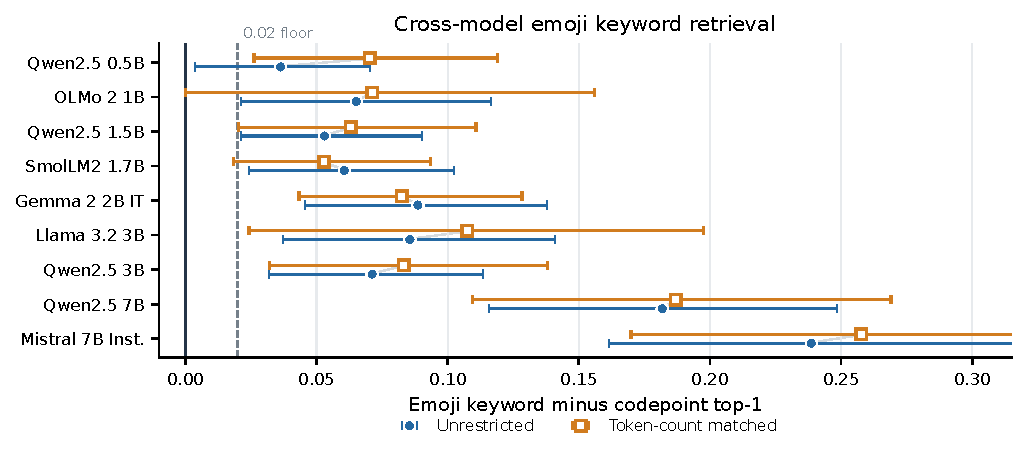
\includegraphics[width=\linewidth]{figures/t19_model_effects.pdf}
  \caption{Emoji keyword-minus-codepoint top-1 effects in the registered roster
  order. Bars are descriptive 95\% item-bootstrap intervals (20,000
  replicates); randomization tests determine the primary decision. The
  $0.02$ floor applies to point estimates. Unrestricted (U) and matched (M)
  analyses use different retained pools, so their magnitudes are not directly
  commensurable. Every displayed point estimate exceeds the floor.}
  \label{fig:model-effects}
\end{figure}

Across models, mean emoji keyword effects were $+0.0979$ unrestricted and
$+0.1084$ matched. Mean official-name effects were larger, $+0.1440$ and
$+0.1718$. Thus, retrieval extends beyond the exact official name, although
the official name remains the stronger key on average. The alternative label
is an exact CLDR keyword, not a human-rated synonym or paraphrase;
training-data co-occurrence could still fully explain the relation.
Descriptively, the unrestricted effect also rises monotonically with
parameter count inside the one family sampled at four sizes (Qwen2.5:
$+0.036$, $+0.053$, $+0.071$, $+0.182$ from 0.5B to 7B). The roster remains
confounded across families, so this ordering is description, not a registered
scale result.

Depth was secondary. The nine recorded fractions were $0, 0.125,\ldots,1.0$;
only $0.75$, $0.875$, and $1.0$ formed the primary window. Across models and
contexts, the unrestricted contrast was $+0.0409$ at depth 0, then $+0.0864$,
$+0.1152$, and $+0.0922$ at the three primary depths, whose mean is the
$+0.0979$ reported above. Individual configurations had different onset and peak
depths, so these data do not support one universal trajectory.

\subsection{A named-symbol control limits the emoji-specific claim}

Non-emoji symbols showed mean keyword effects of $+0.0236$ unrestricted and
$+0.0153$ matched, compared with $+0.0979$ and $+0.1084$ for emoji. The
emoji-minus-symbol point estimate was positive in all nine configurations in both
components. Symbol keywords were heterogeneous: Qwen2.5 3B and 7B were
negative in both components. Official-name retrieval exceeded keyword retrieval
for symbols in 9/9 configurations in both components, with mean symbol official-name effects
of $+0.0750$ and $+0.0821$ (Figure \ref{fig:symbol-boundary}).

\begin{figure}[t]
  \centering
  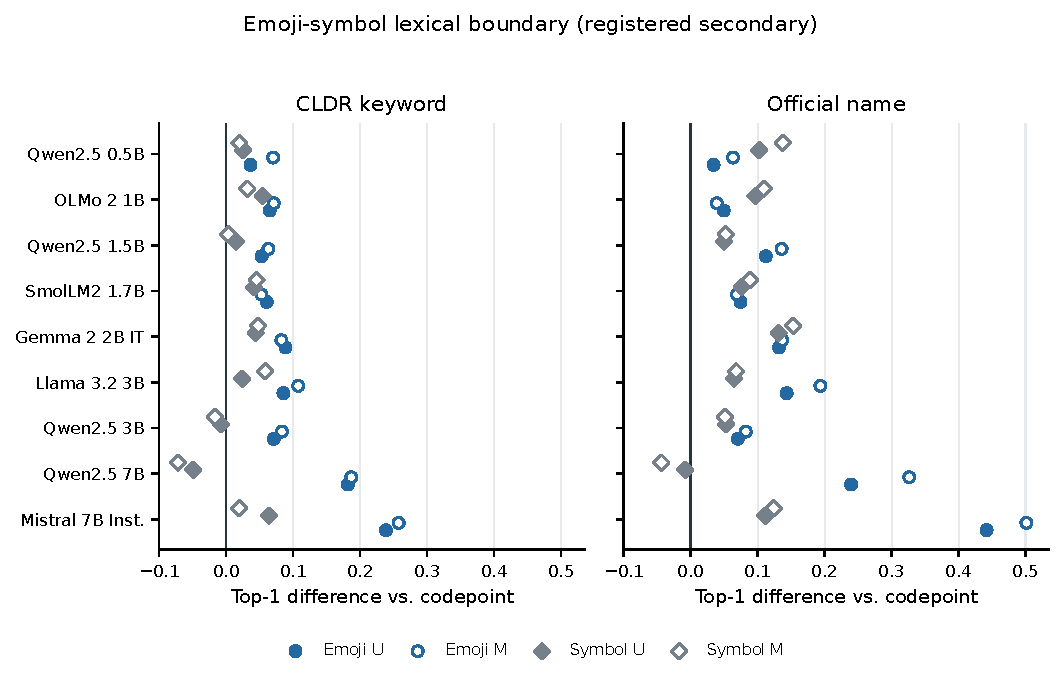
\includegraphics[width=\linewidth]{figures/t19_emoji_symbol_boundary.pdf}
  \caption{Registered secondary comparison. Each row shows unrestricted (U)
  and token-count-matched (M) effects for the same prespecified model. Official-name
  retrieval is not exclusive to emoji; disjoint-keyword effects are
  stronger and more consistent for the prespecified emoji panel. Glyph category,
  frequency, label quality, and token identity are not exchangeable, so this
  is a boundary result rather than an emoji-only semantic claim.}
  \label{fig:symbol-boundary}
\end{figure}

This comparison cannot establish an emoji-specific faculty. The panels are
not matched on training frequency, lexical specificity, Unicode category,
visual familiarity, or token identity. Its role is to prevent the incorrect
inference that only emoji acquire readable names.

\subsection{No prespecified late-component site passes both causal criteria}

Before intervention, the final-hidden glyph endpoint on the 192-item causal
evaluation set was $E_s=0.07292$ (keyword top-1 $0.07292$, i.e.\ 14 of 192
items; codepoint top-1 $0$); the zero-hook engineering check reproduced this
baseline identically at all six sites. The
$0.02$ decision floor was therefore 27\% of this baseline contrast, and the
design contained no positive intervention control that calibrated attainable
adjusted necessity at the primary sites. All six causal sites passed
their engineering checks: zero-hook and
remove-restore conditions reproduced the baseline final hidden state with
exactly zero RMS difference. Bitwise equality is the expected pass state, not
a numerical coincidence: baseline forwards reuse the exact intervention batch
geometry, so any nonzero residue would indicate hook or batching infidelity. Nevertheless, neither primary block-24 site
passed. Block-24 attention had adjusted necessity $0.0000$ and sufficiency
$-0.00521$; block-24 MLP had $+0.00521$ and $0.0000$. Their site IUT values
were $1.0$ and $0.74912$, respectively. None of the six sites passed both
components (Figure \ref{fig:causal}; exact values in Appendix
\ref{app:causal}).

\begin{figure}[t]
  \centering
  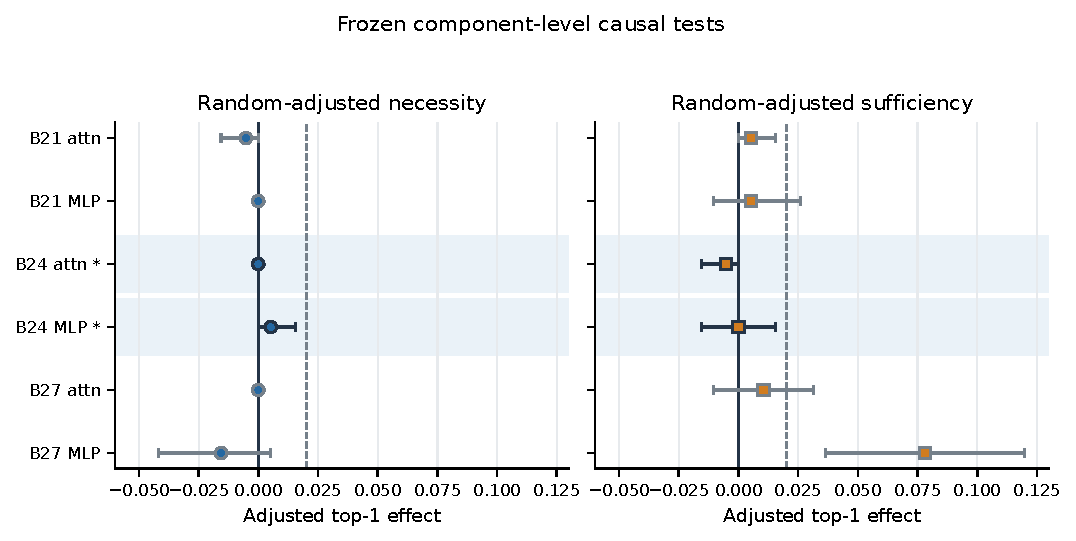
\includegraphics[width=\linewidth]{figures/t19_causal_sites.pdf}
  \caption{Random-adjusted causal effects with descriptive 95\% item-bootstrap
  intervals over 192 emoji held out from T19-L. Shaded rows and asterisks mark the two
  primary block-24 sites. Solid vertical lines show zero; dashed lines show the
  registered $0.02$ effect-size floor. No site has both necessity and sufficiency above the
  floor with positive lower bounds.}
  \label{fig:causal}
\end{figure}

The secondary block-27 MLP patch produced adjusted sufficiency $+0.07812$
(95\% interval $[+0.03646,+0.11979]$; one-sided $p=0.00009$, uncorrected,
with twelve such component tests run in total). Necessity was $-0.01562$ (interval
$[-0.04167,+0.00521]$, $p=0.96895$), giving a site IUT of $0.96895$.
The learned patch raised keyword top-1 from $1/192$ to $4/192$ while lowering
codepoint self-retrieval from $192/192$ to $180/192$. The keyword gain accounts
for 3 of the composite endpoint's 15 additional correct contrasts; the
remaining 12 arise from lost codepoint self-retrieval. This pattern is
consistent with broad representational disruption and does not identify a
necessary keyword mechanism.

\section{Discussion}

The two arms answer different questions. Under a fixed text-only readout,
T19-L recovers the same item across raw emoji and a word-disjoint CLDR keyword
more reliably than across raw emoji and a literal codepoint string. Exact
token-count matching makes a pure length account insufficient. The symbol
panel places the official-name effect within a broader Unicode phenomenon and
shows graded, rather than categorically emoji-only, keyword breadth.

T19-C evaluates a narrower mechanistic hypothesis: one shared rank-8 late
attention or MLP component learned from a source set and tested on a separate
evaluation set. None of the prespecified sites passes joint necessity and
sufficiency. Aggregate linear readability therefore remains compatible with
the absence of a single shared rank-8 late component. Distributed, redundant,
nonlinear, and item-private accounts remain open.

The block-27 MLP asymmetry sharpens that distinction. Its patch moved the
composite endpoint mainly by degrading codepoint self-retrieval. Requiring
necessity, sufficiency, random-subspace adjustment, restoration, and a disjoint
evaluation set prevents that isolated movement from being upgraded to a
circuit claim.

\section{Limitations and broader impact}

\paragraph{Measurement.}
CLDR keywords are standardized annotations, not human judgments of synonymy,
natural naming, specificity, or familiarity. Retrieval is nearest-neighbor
geometry at selected suffix tokens, not generation or task behavior. Inputs
are Unicode text; no rendered glyph is perceived. Exact token-count matching
does not match token identities or equalize tokenizer construction.

\paragraph{Generalization.}
The nine model--tokenizer configurations are a prespecified,
convenience-constrained roster
spanning several families and sizes \citep{yang2024qwen25,groeneveld2024olmo,
dubey2024llama3,gemmateam2024gemma2,jiang2023mistral,benallal2025smollm2}. Model
family, parameter count, training data, tokenizer, and instruction tuning are
confounded, so the study supports neither a scale law nor a model-population
estimate. Exact emoji surfaces are not pretraining-novel. The symbol panel is
repository-text-fresh but not a pretraining holdout and is not exchangeable
with the emoji panel.

\paragraph{Mechanism.}
The negative causal result covers one Llama 3.2 3B checkpoint, rank 8, one
carrier and distance, two primary and four secondary sites, and one
final-hidden endpoint. That endpoint has less aggregation and lower baseline
signal than the observational primary. Its exact engineering checks verify
hook fidelity, while the absence of a prespecified positive intervention
control leaves power and attainable dynamic range uncalibrated. The result
does not exclude other causal representations: optimized interchange
subspaces \citep{geiger2024das,wu2023boundless}, sparse feature bases
\citep{bricken2023monosemanticity,cunningham2024sparse}, distributed
multi-site carriers, and nonlinear readouts were not evaluated.
A future study should preregister such a positive control together with those
alternatives on a new source/evaluation split rather than selecting a method
on the present evaluation set.

\paragraph{Reproducibility and impact.}
The anonymous compact archive binds configurations, selections, summaries,
tests, validators, license notices, and the rendered paper. It omits
model-dependent raw arrays retained in execution scratch. Exact acquisition
duration and peak memory were not receipt-bound and are not reconstructed
after the fact. Better Unicode auditing could reveal hidden representation
failures in multilingual or social-media systems. Conversely, treating CLDR
correspondence as a person's meaning, sentiment, culture, or identity could
erase contextual variation and enable unjustified profiling. The measurements
should not be used for such inference. No personal data, human subjects, or
user messages are used.

\section{Conclusion}

Across nine prespecified model--tokenizer configurations, raw atomic emoji
retrieve word-disjoint CLDR keywords better than literal codepoints after
exact four-view token-count matching. A named-symbol comparison bounds the
specificity of that observation. A separately partitioned causal experiment
finds no primary rank-8 late component that is jointly necessary and
sufficient. Together, these results establish broad lexical readability under
a text-only metric and reject the prespecified sparse late-component account.
Visual understanding and a general emoji circuit remain outside the evidence.

\bibliographystyle{plainnat}
\bibliography{references}

\clearpage
\appendix

\section{Exploration path and decision lineage}
\label{app:lineage}

T19-L is the nineteenth internal study label in a longer audit trail, not a
concept that readers are expected to know in advance. The concise lineage
below includes only results that changed the next design decision. These
studies motivated T19-L. They are not pooled with its preregistered
primary, and their exploratory or failed-confirmation status is unchanged.

Figure \ref{fig:lineage} groups the sequence by the question each stage
resolved. The labels trace design decisions rather than a cumulative evidence
pipeline.

\begin{figure}[t]
  \centering
  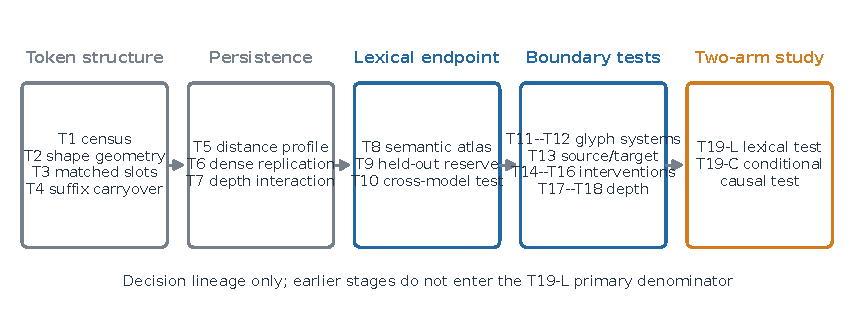
\includegraphics[width=\linewidth]{figures/t19_lineage.pdf}
  \caption{Exploration-to-confirmation lineage. Early studies exposed
  token-structure and persistence explanations; later studies narrowed the
  endpoint and causal test. Arrows record design decisions, not evidence
  pooling. Only the T19-L primary supports the confirmatory lexical claim in
  this paper.}
  \label{fig:lineage}
\end{figure}

\paragraph{Initial screen and matched controls (baseline and Milestone 2).}
A colored-shape steering screen produced 25 positive results among 36
layer--seed--dose configurations. An exact tokenization-matched follow-up
supported one tested layer contrast and failed to support the other. We made
tokenization part of the estimand, retained negative configurations, and
stopped treating a pooled steering score as one stable semantic effect.

\paragraph{Token structure and short-range carryover (T1--T4).}
T1, the \emph{multifamily tokenizer census}, found no universal token-count
and prefix match for the fixed colored-shape panel. T2, \emph{multifamily
colored-shape geometry}, yielded no dual-model recurrence at the selected
midpoint. T3, \emph{five-family matched-slot geometry}, found recurrence only
in OLMo, where the exact shared slot token was already a sufficient
explanation. T4, \emph{common-suffix carryover}, showed that the OLMo pattern
persisted one common token later. The sequence converted tokenizer structure
from a nuisance variable into an explicit competing explanation.

\paragraph{Persistence, depth, and the lexical turn (T5--T8).}
T5, the \emph{carrier-distance profile}, and T6, the \emph{dense CUDA
carrier-distance replication}, both failed their prespecified
distance-attenuation conjunctions. T7, \emph{Mistral base
depth-by-distance}, passed an early-versus-late interaction in a model and
endpoint selected after T6, so it remained prospective within that configuration
rather than independent confirmation. T8, the \emph{Mistral semantic atlas},
then mapped 842 discovery emoji and found a large descriptive
name-over-codepoint contrast. That atlas supplied the endpoint later tested on
the untouched T9 reserve.

\paragraph{Lexical exploration and failed reserves (T9--T12).}
A held-out Mistral configuration first supported name-over-codepoint retrieval. A
nine-configuration follow-up retained statistical signal and failed its
registered cross-model effect-size rule. Broader glyph-system exploration then suggested
Unicode-composition hypotheses; neither survived testing on separately
reserved items. We kept both failures, dropped the generic composition claim,
and returned to a narrower lexical question.

\paragraph{Specificity decomposition and first causal localization (T13--T14).}
T13 separated structured source directions from generic target susceptibility
on already exposed panels and remained exploratory. T14 then paired a signed
six-model intervention grid with a separately specified selected-site test.
The broad response pattern was heterogeneous across model, depth, source form,
null family, and sign; the selected Llama component failed the joint causal
criterion on a new evaluation set. This combination motivated the
response-shape tests and stricter causal separation in T15--T16.

\paragraph{Readable responses and unsuccessful causal tests (T15--T16).}
An emoji--word response pattern replicated prospectively, and prespecified
forced-choice associations were detectable. Yet a subspace intervention and
a multi-layer transplantation each failed their stronger causal criteria. This
separated readout from implementation and motivated the present joint
necessity--sufficiency criterion.

\paragraph{Depth mapping and fresh confirmation (T17--T18).}
Across 292 previously exposed atomic emoji, name-minus-codepoint retrieval was
positive in all nine model configurations at middle-to-late depths. Peaks were
model-specific, and final item retrieval (9/9) did not require consistent
whole-representation CKA alignment (4/9 configurations). We therefore
prespecified a common late window, replaced the population, and made no shared-transition or
universal-manifold claim. On 192 repository-fresh composite emoji, the
official-name contrast then
passed in 4/4 core configurations and 8/9 configurations overall after exact token-count
matching. This justified asking whether the relation extends beyond the
official short name, while adding a named non-emoji control and reserving new
item sets for causality. This T18 composite set is distinct from the 192
atomic emoji in the T19-C evaluation set.

\paragraph{T19-L and T19-C (current confirmatory and conditional arms).}
T19-L replaces the sole label endpoint with a word-disjoint CLDR keyword and
adds literal-codepoint and named-symbol boundaries. T19-C tests the prespecified
rank-8 component account on disjoint source and evaluation sets. The present
paper reports the resulting pair of differently gated results: broad lexical
retrieval passes, while the simple late-component mediator does not.

This lineage explains why the final design contains four text views, exact
token-count strata, a non-emoji symbol panel, three disjoint item sets, and a
necessity--sufficiency intersection. It also explains what is absent: no
favorable prior layer, glyph system, or causal site was promoted into the
T19-L primary. Only that prespecified primary supports the paper's confirmatory
lexical claim.

\section{Prespecified model roster}
\label{app:models}

Table \ref{tab:models} reports the exact model artifacts and revisions used by
the prespecified observational roster. The Llama role uses the pinned BF16 mirror
artifact specified by the protocol. Despite its \texttt{mlx-community}
identifier, the recorded run loaded its safetensors through the
Transformers/CUDA backend; we make no upstream bit-identity claim. Model cards
and upstream license terms are part of the submission-archive license audit.
The cards declare Apache-2.0 for the Qwen2.5 0.5B, 1.5B, and 7B configurations, OLMo,
SmolLM2, and Mistral; Qwen2.5 3B uses the non-commercial Qwen Research
License, Gemma uses the Gemma Terms of Use, and the Llama mirror uses the
Llama 3.2 Community License. No checkpoint or tokenizer file is redistributed.

\begin{table}[H]
\centering
\scriptsize
\setlength{\tabcolsep}{3.5pt}
\begin{tabular}{lll}
\toprule
Role & Artifact identifier & Revision \\
\midrule
Qwen2.5 0.5B base & \texttt{Qwen/Qwen2.5-0.5B} & \texttt{060db6499f32} \\
OLMo 2 1B base & \texttt{allenai/OLMo-2-0425-1B} & \texttt{a1847dff3500} \\
Qwen2.5 1.5B base & \texttt{Qwen/Qwen2.5-1.5B} & \texttt{8faed761d45a} \\
SmolLM2 1.7B base & \texttt{HuggingFaceTB/SmolLM2-1.7B} & \texttt{effd688a1292} \\
Gemma 2 2B IT & \texttt{google/gemma-2-2b-it} & \texttt{299a8560bedf} \\
Llama 3.2 3B base & \texttt{mlx-community/Llama-3.2-3B-bf16} & \texttt{60a99aaf4316} \\
Qwen2.5 3B base & \texttt{Qwen/Qwen2.5-3B} & \texttt{3aab1f1954e9} \\
Qwen2.5 7B base & \texttt{Qwen/Qwen2.5-7B} & \texttt{d14972939875} \\
Mistral 7B Inst. v0.3 & \texttt{mistralai/Mistral-7B-Instruct-v0.3} & \texttt{c170c708c41d} \\
\bottomrule
\end{tabular}
\caption{Pinned artifact identifiers and the first 12 hexadecimal characters
of their complete pinned revisions. Full revisions are stored in the
submission manifest.}
\label{tab:models}
\end{table}

\section{Exact observational results}
\label{app:observational}

\begin{table}[H]
\centering
\small
\begin{tabular}{lrrrc}
\toprule
Model configuration & U effect & M effect & Model IUT $p$ & Pass \\
\midrule
Qwen2.5 0.5B & 0.0364 & 0.0702 & 0.00055 & yes \\
OLMo 2 1B & 0.0652 & 0.0712 & 0.00135 & yes \\
Qwen2.5 1.5B & 0.0530 & 0.0631 & 0.00185 & yes \\
SmolLM2 1.7B & 0.0606 & 0.0528 & 0.00005 & yes \\
Gemma 2 2B IT & 0.0886 & 0.0825 & 0.00005 & yes \\
Llama 3.2 3B & 0.0856 & 0.1075 & 0.00135 & yes \\
Qwen2.5 3B & 0.0712 & 0.0833 & 0.00005 & yes \\
Qwen2.5 7B & 0.1818 & 0.1869 & 0.00005 & yes \\
Mistral 7B Inst. & 0.2386 & 0.2577 & 0.00005 & yes \\
\bottomrule
\end{tabular}
\caption{Exact reporting values for the registered emoji
keyword-minus-codepoint endpoint. U is unrestricted; M is exact four-view
token-count matched. The model IUT is the maximum component randomization
$p$-value.}
\label{tab:observational}
\end{table}

Matched emoji counts ranged from 31 to 41. The matched component retained at
least 63 observational items total in every configuration, with at least 31 emoji and
32 symbols; the unrestricted component used all 55 emoji and 55 symbols. The
acquisition comprised $9\times110\times4\times2=7{,}920$ batch-one forwards
(configurations $\times$ items $\times$ views $\times$ carriers). Four
distances and nine depths produced $7{,}920\times4\times9=285{,}120$ readout
vectors in 45 sealed shards.

\section{Exact causal results}
\label{app:causal}

\begin{table}[H]
\centering
\scriptsize
\setlength{\tabcolsep}{3pt}
\begin{tabular}{llcrrrrr}
\toprule
Block & Site & Primary & $N_s$ & $p_N$ & $S_s$ & $p_S$ & Site IUT \\
\midrule
21 & attention & no  & -0.00521 & 1.00000 &  0.00521 & 0.49983 & 1.00000 \\
21 & MLP       & no  &  0.00000 & 1.00000 &  0.00521 & 0.49760 & 1.00000 \\
24 & attention & yes &  0.00000 & 1.00000 & -0.00521 & 1.00000 & 1.00000 \\
24 & MLP       & yes &  0.00521 & 0.49989 &  0.00000 & 0.74912 & 0.74912 \\
27 & attention & no  &  0.00000 & 1.00000 &  0.01042 & 0.31511 & 1.00000 \\
27 & MLP       & no  & -0.01562 & 0.96895 &  0.07812 & 0.00009 & 0.96895 \\
\bottomrule
\end{tabular}
\caption{Random-adjusted necessity ($N_s$) and sufficiency ($S_s$). All six
engineering checks passed. Holm correction applies across the two primary
sites and did not change either decision; no site passed the component-level
intersection.}
\label{tab:causal}
\end{table}

The causal run used $128\times2=256$ source forwards. For each of 192
evaluation items, three baseline-view forwards plus two batched intervention
forwards at each of six sites yielded $192\times15=2{,}880$ evaluation
forwards; seven intervention rows per site yielded
$192\times6\times7=8{,}064$ rows. Each of 12 component tests used 99,999 sign flips and
20,000 item-bootstrap replicates. An independent validator rehashed source and
evaluation arrays, reconstructed all 12 tests and intervals, verified learned
and random subspace relations, and reproduced six engineering passes and zero
positive sites.

\section{Execution, licensing, and artifact boundary}
\label{app:artifact}

Both observational and causal acquisition used a fixed Transformers/CUDA
BF16 environment and an NVIDIA GeForce RTX 5090. Model artifacts, tokenizer replay
receipts, selection files, analysis summaries, randomization seeds, bootstrap
seeds, and validators are checksum-bound. Figure inputs in the paper are only
the compact validated model-configuration and causal-site JSON summaries; a generated
manifest hashes both inputs and every plotted PDF/PNG output.

The anonymous evidence archive is a deterministic whitelist-only zip. Its
manifest records every payload path, byte count, and SHA-256; a validator
rejects unsafe paths, author or local-path tokens, model-weight formats, and
raw array formats. The archive includes the paper, compact results, selected
item sets, code, validation receipts, and paired license/compute/ethics reports.
It omits model-dependent activation arrays, learned causal subspaces, the full
intervention ledger, model weights, and tokenizer files. Those raw scientific
objects remain bound by run receipts in execution scratch. The package thus
supports compact-summary and figure audit, not self-contained raw replay.

The observational acquisition used 7,920 batch-one forwards and produced
285,120 readout vectors. Causal acquisition used 256 source forwards, 2,880
evaluation forwards, and 8,064 intervention rows. No training or generation
was performed. Exact wall-clock time, peak memory, energy use, and total
exploratory compute were not preserved in the T19 compact receipts; the
compute checklist therefore remains negative rather than substituting older
run timings.

Selected Unicode 17 and CLDR 48.2 rows are used under Unicode License v3 and
travel with its copyright and permission notice. New project code is
Apache-2.0. Restricted checkpoint assets are referenced by pinned revision and
upstream terms rather than redistributed. In particular, the Qwen2.5 3B configuration
is used only for non-commercial research under the Qwen Research License.

We reviewed the study against the NeurIPS Code of Ethics. It uses no human
participants, personal data, private messages, or scraped user content. LLM
coding and research assistants supported protocol drafting, code generation,
manuscript editing, and one author-side fresh-eyes review; they did not provide
labels, choose outcomes after T19 execution, or serve as the scientific
evaluator. The authors retained execution authority and approved the prespecified
endpoints and final claims; numerical evidence and validators were
checksum-bound.

\section*{NeurIPS Paper Checklist}

\begin{enumerate}

\item {\bf Claims}
  \item[] Question: Do the main claims made in the abstract and introduction accurately reflect the paper's contributions and scope?
  \item[] Answer: \answerYes{}
  \item[] Justification: Sections 1, 5, and 6 separate the positive observational result, the negative registered causal result, and their bounded interpretation.

\item {\bf Limitations}
  \item[] Question: Does the paper discuss the limitations of the work performed by the authors?
  \item[] Answer: \answerYes{}
  \item[] Justification: Section 6 discusses measurement, tokenization, model-roster, causal-scope, archive, and social-interpretation limits.

\item {\bf Theory assumptions and proofs}
  \item[] Question: For each theoretical result, does the paper provide the full set of assumptions and a complete (and correct) proof?
  \item[] Answer: \answerNA{}
  \item[] Justification: The paper reports empirical tests and does not introduce a theoretical result.

\item {\bf Experimental result reproducibility}
  \item[] Question: Does the paper fully disclose all the information needed to reproduce the main experimental results of the paper to the extent that it affects the main claims and/or conclusions of the paper (regardless of whether the code and data are provided or not)?
  \item[] Answer: \answerYes{}
  \item[] Justification: Sections 3 and A--E disclose the complete protocol, prespecified item selections, pinned artifact revisions, seeds, tests, and analysis code, so the main results can be reacquired from public checkpoints. The anonymous package omits retained raw activation arrays; verification is therefore by reacquisition rather than replay, and bit-exact equality across GPU hardware is not claimed.

\item {\bf Open access to data and code}
  \item[] Question: Does the paper provide open access to the data and code, with sufficient instructions to faithfully reproduce the main experimental results, as described in supplemental material?
  \item[] Answer: \answerNo{}
  \item[] Justification: The study depends on code, so N/A is inapplicable. A checksum-bound anonymous compact artifact is supplied, but no public repository is available at submission and the package omits model-dependent raw arrays required for exact replay. Full code and eligible data are planned for public release after review.

\item {\bf Experimental setting/details}
  \item[] Question: Does the paper specify all the training and test details (e.g., data splits, hyperparameters, how they were chosen, type of optimizer) necessary to understand the results?
  \item[] Answer: \answerYes{}
  \item[] Justification: Section 3 specifies all evaluation sets, observational carriers, distances, and depths, the causal single-carrier distance-1 context, readouts, tests, interventions, and prespecified sites; no model training is performed.

\item {\bf Experiment statistical significance}
  \item[] Question: Does the paper report error bars suitably and correctly defined or other appropriate information about the statistical significance of the experiments?
  \item[] Answer: \answerYes{}
  \item[] Justification: Sections 3.3--3.4 define the randomization, partial-conjunction, sign-flip, Holm, and bootstrap procedures; Figures 2 and 4 label bootstrap intervals as descriptive.

\item {\bf Experiments compute resources}
  \item[] Question: For each experiment, does the paper provide sufficient information on the computer resources (type of compute workers, memory, time of execution) needed to reproduce the experiments?
  \item[] Answer: \answerNo{}
  \item[] Justification: Appendix E identifies the RTX 5090 and BF16 CUDA path and reports forward counts, but exact wall-clock and peak-memory receipts are not in the compact archive.

\item {\bf Code of ethics}
  \item[] Question: Does the research conducted in the paper conform, in every respect, with the NeurIPS Code of Ethics \url{https://neurips.cc/public/EthicsGuidelines}?
  \item[] Answer: \answerYes{}
  \item[] Justification: Section 6 and Appendix E document the completed scope review: no human subjects or personal data, licensed public inputs, explicit representativeness and misuse limits, and disclosed compute-accounting gaps.

\item {\bf Broader impacts}
  \item[] Question: Does the paper discuss both potential positive societal impacts and negative societal impacts of the work performed?
  \item[] Answer: \answerYes{}
  \item[] Justification: Section 6 discusses auditing benefits and the risk of converting standardized lexical correspondence into unjustified cultural, sentiment, or identity inference.

\item {\bf Safeguards}
  \item[] Question: Does the paper describe safeguards that have been put in place for responsible release of data or models that have a high risk for misuse (e.g., pre-trained language models, image generators, or scraped datasets)?
  \item[] Answer: \answerNA{}
  \item[] Justification: The work releases no new pretrained model, scraped dataset, or high-risk capability; it studies public Unicode annotations and existing model checkpoints.

\item {\bf Licenses for existing assets}
  \item[] Question: Are the creators or original owners of assets (e.g., code, data, models), used in the paper, properly credited and are the license and terms of use explicitly mentioned and properly respected?
  \item[] Answer: \answerYes{}
  \item[] Justification: Appendices B and E and the archive license register identify every model and data term. Model/tokenizer files are not redistributed; the Qwen 3B configuration is bounded to non-commercial research; and the Unicode License v3 notice accompanies the derived rows.

\item {\bf New assets}
  \item[] Question: Are new assets introduced in the paper well documented and is the documentation provided alongside the assets?
  \item[] Answer: \answerYes{}
  \item[] Justification: The anonymous artifact includes paired artifact documentation, a machine-readable file manifest, SHA256SUMS, omission boundaries, validation instructions, licenses, prespecified selections, compact evidence, and source code.

\item {\bf Crowdsourcing and research with human subjects}
  \item[] Question: For crowdsourcing experiments and research with human subjects, does the paper include the full text of instructions given to participants and screenshots, if applicable, as well as details about compensation (if any)?
  \item[] Answer: \answerNA{}
  \item[] Justification: The study uses no crowdsourcing or human subjects.

\item {\bf Institutional review board (IRB) approvals or equivalent for research with human subjects}
  \item[] Question: Does the paper describe potential risks incurred by study participants, whether such risks were disclosed to the subjects, and whether Institutional Review Board (IRB) approvals (or an equivalent approval/review based on the requirements of your country or institution) were obtained?
  \item[] Answer: \answerNA{}
  \item[] Justification: The study uses no crowdsourcing, personal data, or human subjects.

\item {\bf Declaration of LLM usage}
  \item[] Question: Does the paper describe the usage of LLMs if it is an important, original, or non-standard component of the core methods in this research? Note that if the LLM is used only for writing, editing, or formatting purposes and does \emph{not} impact the core methodology, scientific rigor, or originality of the research, declaration is not required.
  \item[] Answer: \answerYes{}
  \item[] Justification: Appendix E conservatively discloses assistant support for protocol drafting, code generation, editing, and fresh-eyes review, while separating it from labels, prespecified decisions, execution authority, numerical evidence, and scientific evaluation.

\end{enumerate}


\end{document}
